\begin{scanpage}{0229}{211}
\begin{center}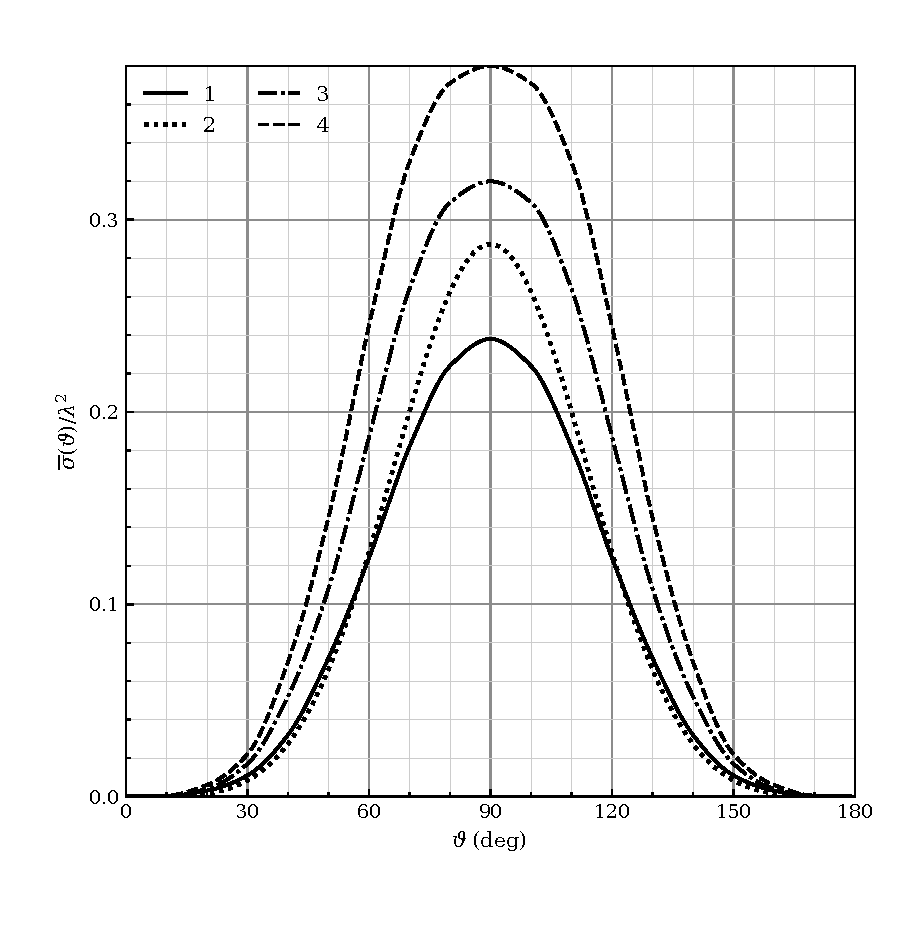
\includegraphics[width=.50\linewidth]{images/recreated/r-0229-fig79.pdf}\par
\begin{minipage}{.78\linewidth}
Figure 79. A comparison of the diagrams for the effective scattering area of a half-wave vibrator calculated by various methods.
\par Curve 1 was calculated by Tai [87] by the variational method;
\par Curve 2 was calculated on the basis of Equation (34.12);
\par Curve 3 was calculated by the method of induced emf (in the work of Van Vleck [86]);
\par Curve 4 was calculated by Van Vleck [86] by the method of integral equations.
\end{minipage}\end{center}
In the cited references, the fringing field was calculated by the direct integration of the current. In order to determine the current, various approximation methods were used. In the variational method [87] a functional was constructed for this purpose which was stationary in respect to small current variations. Then the current was sought in the form of some function containing undetermined constants. These constants were found from the condition of the functional's stationarity. This method enables one to rather easily
\end{scanpage}
